\documentclass[dvipdfmx]{jarticle}
\pagestyle{empty}
\usepackage{tikz}
\usetikzlibrary{shapes,calc}
\begin{document}
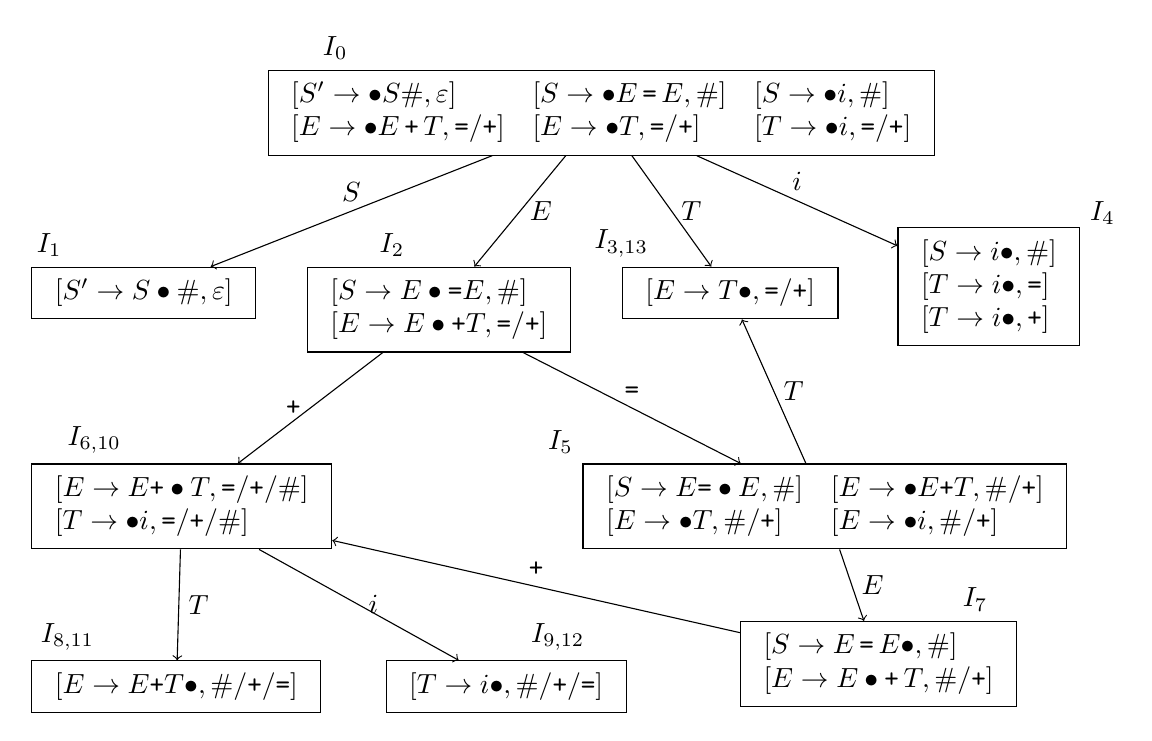
\begin{tikzpicture}
  \node[draw,rectangle,label=170:{$I_0$},anchor=north west] (I0) at (0,0) {
    $\begin{array}{lll}
      [S'\rightarrow\bullet S\#,\varepsilon] & [S\rightarrow\bullet E\,\texttt{=}\,E,\#] & [S\rightarrow\bullet i,\#]\\\relax
      [E\rightarrow\bullet E\,\texttt{+}\,T,\texttt{=}/\texttt{+}] & [E\rightarrow\bullet T,\texttt{=}/\texttt{+}] & [T\rightarrow\bullet i,\texttt{=}/\texttt{+}]
    \end{array}$
  };

  \node[draw,rectangle,label=160:{$I_1$},anchor=north west] (I1) at (-3,-2.5) {
    $\begin{array}{l}
      [S'\rightarrow S\bullet\#,\varepsilon]
    \end{array}$
  };

  \node[draw,rectangle,label=120:{$I_2$},anchor=north west] (I2) at (0.5,-2.5) {
    $\begin{array}{l}
      [S\rightarrow E\bullet\texttt{=}E,\#]\\\relax
      [E\rightarrow E\bullet\texttt{+}T,\texttt{=}/\texttt{+}]
    \end{array}$
  };

  \node[draw,rectangle,label=160:{$I_{3,13}$},anchor=north west] (I313) at (4.5,-2.5) {
    $\begin{array}{l}
      [E\rightarrow T\bullet,\texttt{=}/\texttt{+}]
    \end{array}$
  };

  \node[draw,rectangle,label=30:{$I_4$},anchor=north west] (I4) at (8,-2) {
    $\begin{array}{l}
      [S\rightarrow i\bullet,\#]\\\relax
      [T\rightarrow i\bullet,\texttt{=}]\\\relax
      [T\rightarrow i\bullet,\texttt{+}]
    \end{array}$
  };

  \node[draw,rectangle,label=170:{$I_5$},anchor=north west] (I5) at (4,-5) {
    $\begin{array}{ll}
      [S\rightarrow E\texttt{=}\bullet E,\#] & [E\rightarrow \bullet E\texttt{+}T,\#/\texttt{+}]\\\relax
      [E\rightarrow \bullet T,\#/\texttt{+}] & [E\rightarrow \bullet i,\#/\texttt{+}]
    \end{array}$
  };

  \node[draw,rectangle,label=140:{$I_{6,10}$},anchor=north west] (I610) at (-3,-5) {
    $\begin{array}{l}
      [E\rightarrow E\texttt{+}\bullet T,\texttt{=}/\texttt{+}/\#]\\\relax
      [T\rightarrow \bullet i,\texttt{=}/\texttt{+}/\#]
    \end{array}$
  };

  \node[draw,rectangle,label=30:{$I_7$},anchor=north west] (I7) at (6,-7) {
    $\begin{array}{l}
      [S\rightarrow E\,\texttt{=}\,E\bullet,\#]\\\relax
      [E\rightarrow E\bullet\texttt{+}\,T,\#/\texttt{+}]
    \end{array}$
  };

  \node[draw,rectangle,label=160:{$I_{8,11}$},anchor=north west] (I811) at (-3,-7.5) {
    $\begin{array}{l}
      [E\rightarrow E\texttt{+}T\bullet,\#/\texttt{+}/\texttt{=}]
    \end{array}$
  };

  \node[draw,rectangle,label=60:{$I_{9,12}$},anchor=north west] (I912) at (1.5,-7.5) {
    $\begin{array}{l}
      [T\rightarrow i\bullet,\#/\texttt{+}/\texttt{=}]
    \end{array}$
  };

  \path[->] (I0) edge [above] node {$S$} (I1) (I0) edge [right] node {$E$} (I2)
            (I0) edge [right] node {$T$} (I313) (I0) edge [above] node {$i$} (I4);
  \path[->] (I2) edge [left] node {$\texttt{+}$} (I610) (I2) edge [above] node {$\texttt{=}$} (I5);
  \path[->] (I5) edge [right] node {$T$} (I313) (I5) edge [right] node {$E$} (I7);
  \path[->] (I7) edge [above] node {$\texttt{+}$} (I610);
  \path[->] (I610) edge [right] node {$T$} (I811) (I610) edge [right] node {$i$} (I912);

\end{tikzpicture}
\end{document}